\section{Introdução e Justificativas}\label{Intro}


%=============================================================================
% 							INTRODUÇÃO
%=============================================================================

%GFC E QUESTIONAMENTO DO INVESTIMENTO COMO CAUSA CAUSANS
PALAVRA INICIAL 
Os impactos sócio-econômicos da Crise Financeira Global (CFG) são imensuráveis, mas algumas das mudanças sobre a teoria econômica já podem ser tateadas. Se, por um lado, abalou a macroeconomia ortodoxa ao ponto da política fiscal estar sendo repensada, por outro, redirecionou algumas pautas na heterodoxia. Distribuição e desigualdade, temas tão caros a esta última tradição, ganharam novo fôlego enquanto parte da literatura passou a destacar o consumo como um dos possíveis motores de crescimento \cite{brochier_macroeconomics_2017}. Desse modo, umas das consequências da CGF é a reavaliação do investimento das firmas enquanto  ``a causa das causas''. Paralelamente, verificou-se um crescente interesse nas implicações macroeconômicas do investimento residencial\footnote{E isso é verificado até na literatura ortodoxa. Inspecionando modelos DSGE que incluem investimento residencial, \textcite{iacoviello_housing_2010} conclui que um melhor entendimento dos impactos deste gasto se faz necessária para a compreensão das flutuações macroeconômicas. } \cite{fiebiger_semi-autonomous_2018}. 

Neste ponto, cabe mencionar o ineditismo de \textcite{green_follow_1997} e \textcite{leamer_housing_2007} --- e revisitado em \textcite{leamer_housing_2015} e por \textcite{fiebiger_trend_2017} --- ao lançar luz sobre a importância do investimento residencial na determinação dos ciclos econômicos antes da crise dos \textit{subprimes}. Ao avaliar o caso norte-americano, \textcite{green_follow_1997} conclui que o investimento residencial possui uma capacidade preditiva maior que o investimento das firmas, mas que isso não implica no estabelecimento de uma relação causal. Na tentativa de compreender tais resultados, afirma:

\begin{quote}
	
	[P]erhaps residential investiment, like stock prices and interest rates, is a good predictor of GDP because it is a series that reflects \textbf{foward looking behavior}. Presumably households will not increase their expenditures on housing unless they expect to prosper in the future. Building a house is a natural mechanism for doing this. Thus, the series can do a good job of predicting GDP without necessarily causing GDP.
	\cite[p.~267, grifos adicionados]{green_follow_1997}
\end{quote}
\textcite{leamer_housing_2007}, por sua vez, avança em direção a relação de causalidade entre este gasto e o PIB. Grosso modo, afirma que a construção de novos imóveis implica em maior consumo de bens duráveis e, portanto, trata-se de um ciclo decorrente do \textit{volume} e não do preço dos imóveis. MAIS REFERÊNCIAS SOBRE EUA.

Além disso, parte da literatura empírica recente também têm lançado luz sobre a importância deste gasto para o ciclo econômico. \textcite{alvarez_does_2010}, por exemplo, concluem que tal tipo de investimento antecede o ciclo econômico para o caso de espanhol e resultados semelhantes podem ser encontrados para França \cite{ferrara_cyclical_2010}, Espanha  e Itália enquanto o caso alemão apresenta uma dinâmica distinta \cite{ferrara_common_2010}. 
Outros estudos, por sua vez, têm enfatizado o efeito riqueza sobre o consumo e indicam tais canais de transmissão são mais incidentes, em ordem, sobre Estados Unidos e Grã Bretanha mas mais brandos no caso francês e alemão \cites{sastre_assessment_2010}{chauvin_wealth_2010}{bassanetti_effects_2010}{arrondel_housing_2010}. Por fim, \textcite{huang_is_2018} testam ambas as hipóteses aventadas por Leamer  (predição e causalidade) e concluem que: (i) o investimento residencial não é um mero canal de transmissão da política monetária; (ii) a construção de novos imóveis tem maior capacidade preditiva que os preços; (iii) o preço dos imóveis tem maior influência no longo prazo e (iv) os resultados sobre a relação de causalidade não são conclusivos para todos os países dada heterogeneidade institucional.

A pluralidade de resultados reportada acima sugere que a especificidade institucional de cada país desempenha um papel central nas implicações macroeconômicas do investimento residencial e, portanto, carece de uma análise mais pormenorizada. A título de exemplo, o caso alemão se destoa dos demais em que \textcite{wijburg_alternative_2017} destacam a estabilidade de longo prazo do mercado imobiliário alemão é um contra ponto ao mercado ameriacano\footnote{
	A metodologia utilizada por \textcite{wijburg_alternative_2017} é a das ondas de financeirização em que a última onda iniciou no fim da CFG. Dito isso, os autores negam a ideia de que o mercado imobiliário alemão não é financeirizado uma vez que a financeirização imobiliária pode assumir várias formas.}. 
Apontam que os preços dos imóveis na Alemanha estagnaram enquanto o resto do mundo presenciou um aumento. No entanto, observa-se um movimento recente de aumento nos preços no país, indicando uma maior relevância do tema em um futuro próximo:

\begin{quote}
\textit{On the one hand, the German housing market was one of the few markets in Western Europe that was not severely affected by the global housing boom of the early 2000s. On the other hand, recent developments suggest that the role of finance in the German housing system is \textbf{changing}, but not in the same way as in other countries} \cite[p.~969, grifos adicionados]{wijburg_alternative_2017}
\end{quote}

Neste ponto, cabe destacar a importância da institucionalidade para a compreensão da distinção entro os países bem com as inter-relações entre o mercado imobiliário com o mercado de crédito.

INVESTIMENTO RESIDENCIAL, INSTITUCIONALIDADE: Van guten e cagnin

Dentre os determinantes institucionais, destaca-se: (i) transferência de riscos, dentre eles a securitização que têm aumentado entre os países europeus \cite{european_central_bank_housing_2010}; (ii) disponibilidade de crédito de longo-prazo para as famílias \cite{schwartz_politics_2009}; (iii) duração das hipotecas e existência de um mercado secundário; (iv) determinação  e tipo da taxa de juros das hipotecas (fixa ou flexível); (v) arranjo regulatório sobre reembolso antecipado (contrato ou legislação) e formas de refinanciamento; acesso a linhas de crédito, ou seja, permissividade da retirada do capital próprio (\textit{equity withdrawal contracts})

Dentre os itens elencados anteriormente, destaca-se o acesso a linhas de crédito através das hipotecas que é relevante para o caso norte-americano \cite{cagnin_o_2009} --- e possuem efeitos significativos sobre o ciclo econômico uma vez que impacta o consumo de bens duráveis \cite{leamer_housing_2007} --- mas são mais incomuns nos países europeus \cite[p.~95]{van_gunten_varieties_2018}.

\begin{table}[htb]
	\centering
	\caption{Características institucionais de alguns países europeus}
	\label{Institucional}
	\resizebox{\textwidth}{!}{%
		\begin{tabular}{l|c|c|c|c|c|c}
			\hline \hline\\
			\textbf{Fatores institucionias}                                                              & \multicolumn{1}{c}{\textbf{França}} & \multicolumn{1}{c}{\textbf{Alemanha}} & \multicolumn{1}{c}{\textbf{Itália}} & \multicolumn{1}{c}{\textbf{Holanda}} & \multicolumn{1}{c}{\textbf{Portugal}} & \multicolumn{1}{c}{\textbf{Espanha}} \\\hline
			Maturidade das hipotecas                                                                       & 19                                  & 25-30                                 & 22                                  & 30                                   & 30-40                                 & 30                                   \\\hline
			Tipo de taxa de juros                                                                        & Fixa                                & Fixa                                  & Variável                            & Fixa                                 & Variável                              & Variável                             \\\hline
			\begin{tabular}[c]{@{}l@{}}Reembolso antecipado:\\ Contrato (C)/ Legislação (L)\end{tabular} & C/L                                 & C/L                                   & L                                   & C                                    & L                                     & C/L                                  \\\hline
			\begin{tabular}[c]{@{}l@{}}Retirada de capital próprio \\ (Permissão)\end{tabular}           & Não                                 & Não                                   & Não                                 & Sim                                  & -                                     & Limitado                             \\\hline
			\begin{tabular}[c]{@{}l@{}}Financiamento pelo \\ mercado de capitais\end{tabular}            & 12\%                                & 14\%                                  & 20\%                                & 25\%                                 & 27\%                                  & 45\%                                 \\\hline
			\begin{tabular}[c]{@{}l@{}}Execução hipotecária (\textit{Foreclosure}): \\ duração (meses)\end{tabular}             & 20                                  & 9                                     & 56                                  & 5                                    & 24                                    & 8 \\ \hline\hline                                 
		\end{tabular}%
	}
\caption*{\textbf{Fonte:}  \textcite[p.~94, adaptado e traduzido]{van_gunten_varieties_2018}}
\end{table}



Pontuada a importância deste gasto, cabe inspecionar a forma com que a heterodoxia tratou do tema. Parte significativa desta literatura  --- emergente no pós-crise imobiliária --- centra esforços na conexão deste tipo de gasto com processos mais gerais como a financeirização \cites{aalbers_financialization_2008}{bibow_financialization_2010} enquanto uma fração minoritária o relaciona com as variabilidades de capitalismo e as relações com o \textit{welfare state} \cite{schwartz_politics_2009}. Uma análise alternativa --- apesar de não heterodoxa --- é da  ``hipotecarização'' desenvolvida por \textcite{jorda_great_2014} que destaca a crescente participação das hipotecas nos balanços patrimoniais dos bancos\footnote{\textcite{jorda_great_2014} também destacam que o crédito hipotecário era concedido fora do sistema bancário até os 1900 e isso dificulta a estimação dos dados.} (ver gráfico \ref{GraficoJorda}): 

\begin{quote}
	\textit{To a large extent the core business model of banks in advanced economies today resembles that of real estate funds: banks are borrowing (short) from the public and capital markets to invest (long) into assets linked to real estate.} [...] \textit{looking more deeply at the composition of bank credit, it becomes clear that the rapid growth of \textbf{mortgage lending} to households has been the \textbf{driving force} behind this remarkable change in the composition of banks’ balance sheets} \cite[p.~2, grifos adicionados]{jorda_great_2014}
\end{quote}

Outra contribuição de \citeauthor*{jorda_great_2014} é o desenvolvimento de uma base de dados que contém os subcomponentes dos empréstimos dos bancos para 17 países da OCDE\footnote{São eles: Austria, Bélgica, Canada, Suiça, Alemanha, Dinamarca, Espanha, Finlândia, França, Reino Unido, Itália, Japão, Holanda, Noruega, Portugal, Suécia, Estados Unidos} para os anos de 1870 a 2016 e, portanto, fornece informações ainda não exploradas sobre o sistema bancário. A partir destes dados destacam que os empréstimos tem aumentado a uma velocidade superior ao valor dos ativos e, portanto, verifica-se uma maior alavancagem das famílias apesar do aumento do preço dos imóveis. Portanto, a compreensão do papel das hipotecas bem como do investimento residencial se justifica pelos impactos reais e financeiros sobre o ciclo econômico.
%Adicionalmente, afirmam que a estrutura de crédito tem implicações sobre o ciclo econômico.

%DESENVOLVER MAIS HIPOTECARIZAÇÃO  E FALAR QUE VAI SER INVESTIGADA.


\begin{figure}
	\centering
	\caption{Participação do empréstimo imobiliário no total do balanço patrimonial dos bancos (1880-2016)}
	\label{GraficoJorda}
	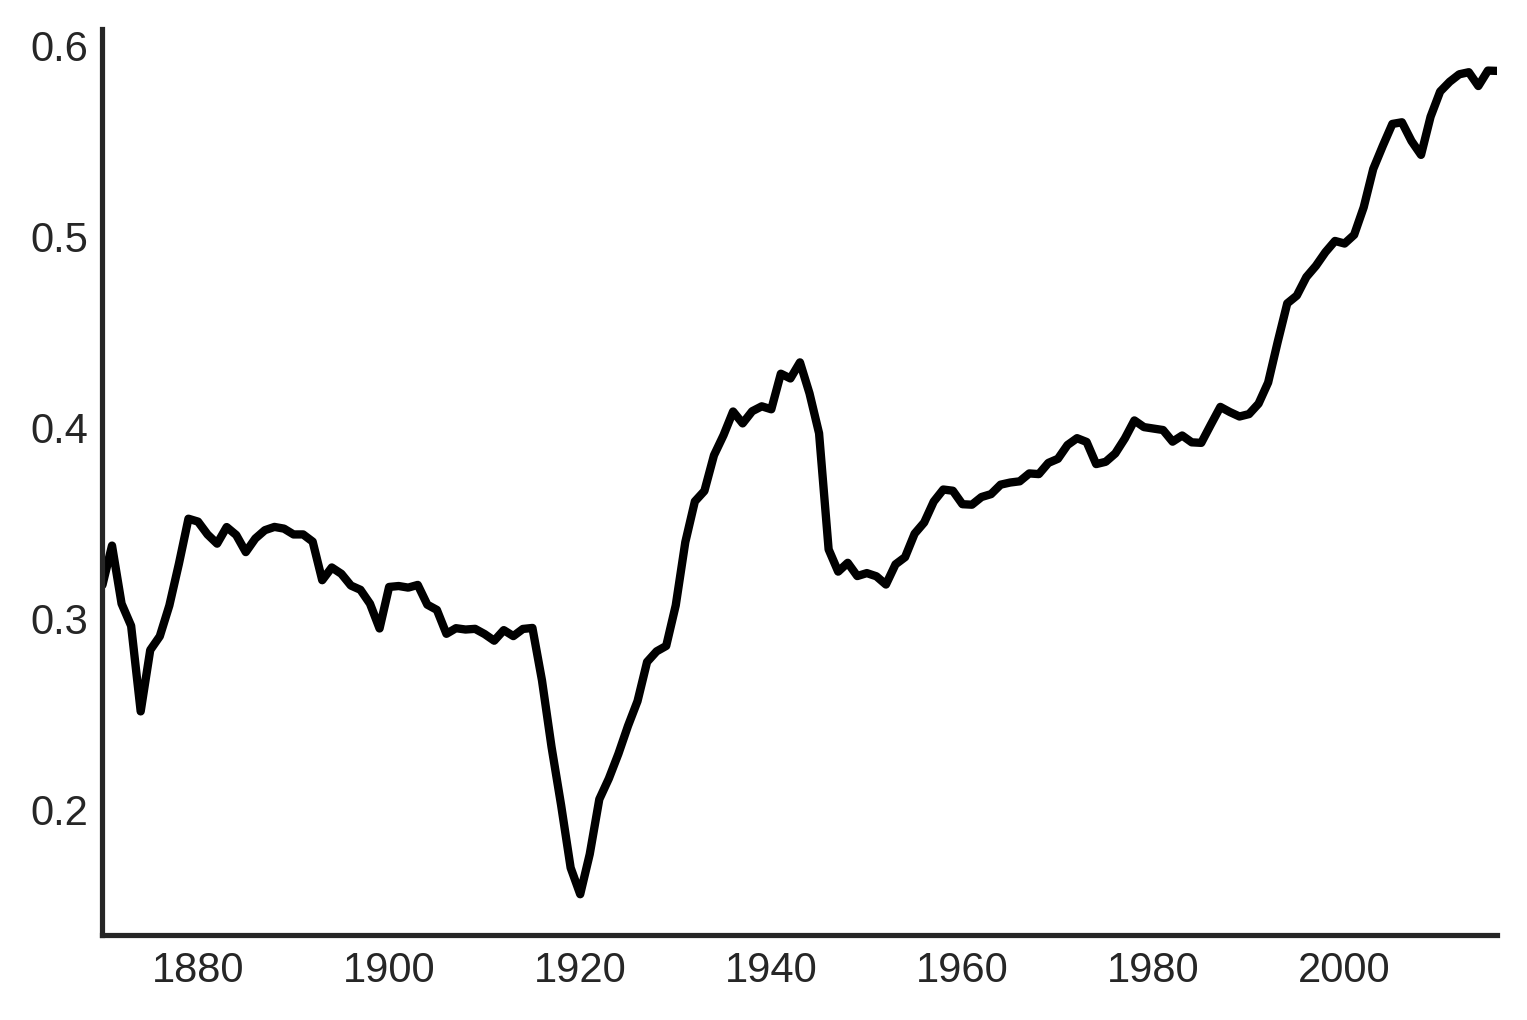
\includegraphics{Jorda_Mean.png}
	\caption*{\textbf{Fonte:}}
\end{figure}

Além disso, a partir da revisão bibliográfica, verificou-se que uma fração pequena da literatura heterodoxa\footnote{
	A título de menção, vale destacar também o trabalho de \textcite{zezza_u.s._2008} em que são investigados os efeitos distributivos sobre o crescimento para a economia norte-americana a partir da metodologia \textit{Stock-Flow Consistent}.}
aborda as relações entre crescimento e investimento residencial que, vale mencionar, não cria capacidade produtiva ao setor privado\footnote{A título de nota, destaca-se que debate ortodoxo sobre desenvolvimento e investimento residencial centrado na década de 60-70 (ver \textcite{arku_housing_2006}) se restringiu em categorizá-lo como um gasto absorvedor de recursos produtivos \cite{solow_importance_1995} e indicava  a possibilidade de um sobreinvestimento residencial \cite{mills_has_1987}. Desse modo, a literatura do supermultiplicador é um contraponto ao \textit{trade-off} apontado por \textcite{solow_importance_1995} uma vez que são os gastos autônomos que lideram o crescimento no longo prazo. 
}. Uma forma de incluir esse gasto nos modelos de crescimento heterodoxos é a de \textcite{da_silveira_investimento_2019} em que os autores utilizam o supermultiplicador sraffiano (SSM em inglês) por estabelecer um papel fundamental aos gastos autônomos que não criam capacidade no crescimento econômico e na acumulação de capital. Na contribuição original de \textcite{serrano_sraffian_1995} e nas apresentações mais recentes \cite{freitas_growth_2015}, o modelo é apresentado de modo bastante parcimonioso para evidenciá-lo como um fechamento alternativo, dentro da tradição da teoria do crescimento liderada pela demanda \cite{serrano_sraffian_2017}. Nesta família de modelos: (i) o grau de utilização converge ao normal no longo prazo; (ii) a distribuição renda tem efeitos de nível apenas e; (iii) a taxa de crescimento converge a taxa de crescimento dos gastos autônomos.

A partir do estabelecimento do SSM, algumas questões são colocadas: quais são esses gastos autônomos e quais seus determinantes? qual o padrão de financiamento e suas consequências? \textcite{pariboni_household_2016} e \textcite{fagundes_role_2017}, por exemplo, avançaram em detalhar o consumo financiado por crédito.  \textcite{brochier_supermultiplier_2018}, por sua vez, incorporam o SSM em uma estrutura contábil mais completa, o arcabouço de consistência entre fluxos e estoques (SFC, na sigla em inglês), para compreender a dinâmica do consumo a partir da riqueza. No entanto, um gasto autônomo tem sido negligenciado: o investimento residencial. 

Uma forma de conectar o investimento residencial com o modelo do supermultiplicador sraffiano é por meio da taxa própria de juros dos imóveis (Taxa Própria) desenvolvida por \textcite{teixeira_crescimento_2015} para avaliar o caso norte americano e é definida como a taxa de juros hipotecária ($r_{mo}$) deflacionada pela inflação dos imóveis ({$\dot p_h$}) de modo que o investimento residencial, autônomo e não criador de capacidade produtiva, cresce a taxa $g_Z$ dada por:
\begin{equation}
g_Z = \phi_0 - \phi_1 \overbrace{\left(\frac{1+r_{mo}}{1+\dot p_h} - 1\right)}^{\text{Taxa Própria}}
\end{equation}
em que os $\phi_i$s são parâmetros e cujo termo em parênteses é a Taxa Própria. O primeiro parâmetro se refere aos determinantes de longo prazo (\textit{e.g.} arranjos institucionais do mercado imobiliários e de crédito) enquanto o segundo capta a demanda por imóveis decorrente das expectativas de ganhos de capital resultantes da especulação com o estoque de imóveis existente e diz respeito ao ciclo econômico.

Em outras palavras, a taxa de juros das hipotecas capta o serviço da dívida para os ``investidores'' (neste caso, famílias) enquanto a variação do preço dos imóveis permite incorporar mudança no patrimonio líquido. Portanto, aufere de modo satisfatório o custo real em imóveis de se comprar imóveis \cite[p.~53]{teixeira_crescimento_2015}. Desse modo, a partir da taxa própria de juros do imóveis é possível revelar importância do investimento residencial para além do ciclo e estendê-la para o longo prazo.  Tal proposta, portanto, lança luz sobre a influência da inflação imobiliária na construção de novos imóveis e, de acordo com o supermultiplicador sraffiano, sobre o produto como um todo. 

Como mencionado anteriormente, a referida taxa própria dos imóveis foi desenvolvida para examinar a bolha de ativos ocorria nos EUA e, portanto, requer uma maior investigação a despeito da aplicabilidade para outros países e este é um dos objetivos desta pesquisa (Ver seção BLA). Além disso, uma vez que a dívida hipotecária é o principal componente do endividamento das famílias, se faz necessária uma melhor compreenssão da conexão entre o investimento residencial com as formas de financiamento e estoques financeiros de forma integrada. Nesses termos, a abordagem \textit{Stock-Flow Consistent} se mostra a mais adequada para este tipo de análise (Ver seção Bla).

SFC E SSM COMO ALTERNATIVA

PERGUNTA

Portanto, a presente investigação estende as contribuições de \textcite{serrano_sraffian_1995} ao incluir o investimento residencial na agenda de pesquisa do supermultiplicador sraffiano tal como em \textcite{da_silveira_investimento_2019}, de \textcite{teixeira_crescimento_2015} ao incorporar o conceito de taxa própria de juros dos imóveis para avaliar a dinâmica de tal gasto autônomo, de \textcite{brochier_supermultiplier_2018} por adicionar um tratamento adequado das relações financeiras no SSM por meio da metodologia SFC 
e a de \textcite{jorda_great_2014} ao lançar luz sobre o processo de ``hipotecarização''. 




\begin{comment}
%=====================================================
%				TEMPORARIAMENTE DESCARTADO
%=====================================================


\end{comment}



